\documentclass{article}

\usepackage{arxiv}

\usepackage[utf8]{inputenc} % allow utf-8 input
\usepackage[T1]{fontenc}    % use 8-bit T1 fonts
\usepackage{hyperref}       % hyperlinks
\usepackage{url}            % simple URL typesetting
\usepackage{booktabs}       % professional-quality tables
\usepackage{amsfonts}       % blackboard math symbols
\usepackage{nicefrac}       % compact symbols for 1/2, etc.
\usepackage{microtype}      % microtypography
\usepackage{lipsum}		% Can be removed after putting your text content
\usepackage{graphicx}
\usepackage{natbib}
\usepackage{doi}
\usepackage{mathtools}
\usepackage{xspace}
\DeclarePairedDelimiter\ceil{\lceil}{\rceil}
\DeclarePairedDelimiter\floor{\lfloor}{\rfloor}



\title{Optimal data splitting in distributed optimization \\for machine learning}

%\date{September 9, 1985}	% Here you can change the date presented in the paper title
%\date{} 					% Or removing it

\author{Gleb Molodtsov
% $ \thanks{Use footnote for providing further
%		information about author (webpage, alternative
%		address)} 
    \\
	Department of Informatics and Applied Maths \\
	Moscow Institute of Physics and Technology\\
	Moscow, Russia\\
	\texttt{molodtsov.gl@phystech.edu} \\
	%% examples of more authors
	\And
	Daniil Medyakov \\
	Department of Informatics and Applied Maths \\
	Moscow Institute of Physics and Technology\\
	Moscow, Russia \\
	\texttt{mediakov.do@phystech.edu} \\
	%% \AND
	%% Coauthor \\
	%% Affiliation \\
	%% Address \\
	%% \texttt{email} \\
	%% \And
	%% Coauthor \\
	%% Affiliation \\
	%% Address \\
	%% \texttt{email} \\
	%% \And
	%% Coauthor \\
	%% Affiliation \\
	%% Address \\
	%% \texttt{email} \\
}

% Uncomment to remove the date
\date{}

% Uncomment to override  the `A preprint' in the header
\renewcommand{\headeright}{Technical Report}
\renewcommand{\undertitle}{Technical Report}
%\renewcommand{\shorttitle}{\textit{arXiv} Template}

%%% Add PDF metadata to help others organize their library
%%% Once the PDF is generated, you can check the metadata with
%%% $ pdfinfo template.pdf

\begin{document}
\maketitle

\begin{abstract}
Distribution of data among different devices taking into account their performance is considered in this article. The network consists of agents forming a star topology. The goal of this work is to get the most favorable ratio for distributed data to the server and local machines. The optimal gradient sliding algorithm and its application to distributed optimization with similarity are used to solve this problem. The system's running times are compared between uniform and optimal distributions. The higher theoretical performance of our solutions is experimentally confirmed. 
\end{abstract}


% keywords can be removed
% \keywords{First keyword \and Second keyword \and More}


\section{Introduction}
The article \citep{kovalev2022optimal} considers the problem of finding an optimal algorithm for distributed optimization.
Consider the features of the formulation of the equation (2) in \citep{kovalev2022optimal}. The network consists of $m$ agents forming a star topology. The first agent is the main node, and the others are connected only to it and are necessary for additional computational power. We are investigating a problem in which we need to minimize the average loss function over some data, and we want to distribute the solution to the objects in our network, where calculations are performed using the edge nodes of the star topology, and copies of all optimization variables and the connection between the cells are made through the main (central) node. For each unit of the network, a loss function is calculated that measures the difference between the parameter vector and the sample vector. Thus, this problem has been reduced to minimizing the following function:
\\
\begin{equation}
    \label{eq:1}
    r(x) = \frac{1}{n} \sum \limits_{i = 1}^{n} f _i(x)
\end{equation}

Consider the pros and cons of this formulation of the problem.
The advantage of \ref{eq:1} is that by applying the gradient descent algorithm, we can solve our minimization problem for an $L$-smooth and $\mu$-strongly-convex function $r$ with complexity $\mathcal{O}(\sqrt{\frac{L}{\mu}})$. This upper bound includes a sum of estimates of local calculations on the edge nodes and their communications with the main node. For some classes of problems (where $k = \frac{L}{\mu}$ is not a large number), this method is acceptable. The disadvantage is that for very large k, the algorithm is inefficient. This happens, for example, with high communication costs.


To avoid this cons we transform the function $r$ to the following form:\\
\begin{equation}
    \label{eq:2}
    r(x) = f_1(x) + \frac{1}{n}\sum\limits_{i = 1}^{n}[f_i(x) - f_1(x)]
\end{equation}

For any $i, f_i$ is a convex function as a loss function of local calculations on an auxiliary node, and $f_i-f_1$ is not convex, but contains communication costs. Thus, we have the task of minimizing an $L$-smooth and $\mu$-strongly-convex function $r$ as the sum of convex and non-convex functions.

For this problem, a modification of the gradient sliding algorithm has been proposed \cite{kovalev2022optimal}, which skips the gradient computation of one function from time to time. All existing gradient sliding algorithms were inapplicable to the problem posed, as they required the convexity of both functions and did not provide optimal upper complexity bounds for both local gradient computation and communication costs. However, this modification of the algorithm fills in the gaps. 

\section{Problem Statement}

Let's consider the accelerated extragradient algorithm (Algorithm 1 in \cite{kovalev2022optimal}). Let us calculate how many operations this algorithm performs per iteration. In line 5, there is one communication, one local computation, one central node calculation, and additional central node computations. In line 6, there is one communication, one local computation, and one central node calculation. Let us make the following notations: $\tau_i$ - the time of one local computation on i-th device, $K$ - the number of iterations, $\tau_{comm}$ - the time for one communication, $k_{some}$ - additional computations of the central node, $n$ - the number of nodes in the network. Then we can write the general running time of the algorithm as:\\
\begin{equation}
    \label{eq:3}
    T_{sum} = 2\cdot\max(\tau_1, \tau_2, ..., \tau_n)\cdot K + 2\cdot K\cdot\tau_{comm} + \tau_1\cdot k_{some}
\end{equation}

Our task is to minimize the time $T_{sum}$. Let's represent the time $\tau_i$ as $\tau_i = \tau_i^{loc}\cdot b_i$, where $\tau_i^{loc}$ is the time spent by the i-th device to process a unit of information submitted to its input, and $b_i$ is the size of dataset submitted to the i-th device. $b_i$ must satisfy the following constraints: $\sum\limits_{i = 1}^{n} b_i = N$, where $N$ is the size of the whole dataset, $\delta = \frac{L}{\sqrt{b_i}}$ or $\delta = \frac{L}{b_i}$ (this estimate is given in \cite{kovalev2022optimal}).
We obtained the following optimization problem:
\begin{equation}
    \label{eq:4}
    \underset{\sum\limits_{i = 1}^{n} b_i = N; \delta = \frac{L}{\sqrt{b_i}}}{min}[ 2\cdot\max(\tau_1^{loc}\cdot b_1, \tau_2^{loc}\cdot b_2, . ., \tau_n^{loc}\cdot b_n)\cdot K + 2\cdot K\cdot\tau_{comm} + \tau_1\cdot k_{some}]
\end{equation}
\section{Problem solution \ref{eq:4}, case $\delta = \frac{L}{\sqrt{b_1}}$}

\subsection{The primary problem of minimization}
In \cite{kovalev2022optimal} the estimates of $K$ and $k_{some}$ are found, namely: \\ $2\cdot K = \mathcal O(max\{1, \sqrt{\frac{L_p}{\mu}}\}log(\frac{1}{\varepsilon})), \tau_1\cdot k_{some} = \mathcal O(max\{1, \sqrt{\frac{L_q}{L_p}}, \sqrt{\frac{L_p}{\mu}}, \sqrt{\frac{L_q}{\mu}}\}\log(\frac{1}{\varepsilon}))$. The value of $\tau_{comm}$ will be determined later. 

Thus, our minimization problem is reduced to:
\begin{equation}
    \label{eq:5}
    \underset{\sum\limits_{i = 1}^{n} b_i = N; \delta = \frac{L}{\sqrt{b_i}}}{min}[(\max(\tau_1^{loc}\cdot b_1, \tau_2^{loc}\cdot b_2, . ., \tau_n^{loc}\cdot b_n) + \tau_{comm}) * \mathcal O(max\{1, \sqrt{\frac{L_p}{\mu}}\log(\frac{1}{\varepsilon})\} 
\end{equation}
\begin{equation}
     \notag
     +
    \mathcal O(max\{1,\sqrt{\frac{L_q}{L_p}}, \sqrt{\frac{L_p}{\mu}}, \sqrt{\frac{L_q}{\mu}}\}\log(\frac{1}{\varepsilon}))]  
\end{equation}

\subsection{Auxiliary problem}
Consider an auxiliary problem:
\begin{equation}
    \label{eq:6}
    \underset{\sum\limits_{i = 1}^{n} b_i = N; \delta = \frac{L}{\sqrt{b_i}}}{min} [\max(\tau_1^{loc}\cdot b_1, \tau_2^{loc}\cdot b_2, ..., \tau_n^{loc}\cdot b_n)]
\end{equation}

Put $\tau_1^{loc}\leq \tau_2^{loc}\leq ... \leq \tau_n^{loc}, b_1\leq b_2\leq ... \leq b_n$. 
And the partition $\{b_i\}_{i = 1}^n$ is arbitrary. We renumber $b_i$ so that a smaller $\tau_i^{loc}$ corresponds to a larger $b_i$ (otherwise, the solution \ref{eq:6} is clearly not optimal, since renumbering will give a smaller value). Minimize $\max(\tau_1^{loc}\cdot b_1, \tau_2^{loc}\cdot b_2, ..., \tau_n^{loc}\cdot b_n)$. Suppose that the largest number must be $\tau_1^{loc}\cdot b_1$. In this case, the partitioning may be such that the first node processes too much information (due to arbitrary partitioning $\{b_i\}_{i = 1}^n$) and the solution \ref{eq:6} will not be optimal. Then we get rid of the maximum at node 1 by making partitions $\{b_i\}$ until we get the maximum at the k-th ($k > 1$) node. This situation may again tell us that the part of the dataset $\{b_i\}_{i = k}^n$ - $b_k$ has too much information compared to the rest and the solution \ref{eq:6} is not optimal. Then we will generate part of the dataset $\{b_i\}_{i = k}^n$ until we get the maximum at the j-th ($j > k$) node, and so on until we get the maximum at the nth node. But then $b_i$ may be about the same, and due to the fact that $\tau_n^{loc}$ takes a large value, the solution will again be optimal. Thus, we obtained that if the maximum is reached at either the 1st or the nth node, then the solution \ref{eq:6} is not minimal. In the first case, because the distribution of $b_i$ is too unequal, and in the second case, because the value of $\tau_n^{loc}$ is large. To avoid these problems, assume that the maximum is reached simultaneously at the 1st and nth nodes. Assume $(\tau_1^{loc}\cdot b_1 = \tau_n^{loc}\cdot b_n)\leq (\tau_2^{loc}\cdot b_2 = \tau_{n-1}^{loc}\cdot b_{n-1})\leq ...$ Then $\max(\tau_1^{loc}\cdot b_1, \tau_2^{loc}\cdot b_2, . ., \tau_n^{loc}\cdot b_n) = \max(\tau_1^{loc}\cdot b_1, \tau_2^{loc}\cdot b_2, ..., \tau_{\ceil{\frac{n}{2}}}^{loc}\cdot b_{\ceil{\frac{n}{2}}})$. Similarly, we assume that the maximum is reached at the 1st and $\ceil{\frac{n}{2}}$ -th nodes, $(\tau_1^{loc}\cdot b_1 = \tau_{\ceil{\frac{n}{2}}}^{loc}\cdot b_{\ceil{\frac{n}{2}}})\leq (\tau_2^{loc}\cdot b_2 = \tau_{\ceil{\frac{n}{2}}-1}^{loc}\cdot b_{\ceil{\frac{n}{2}}-1})\leq . ..$. Continuing in this way, we obtain that $\tau_1\cdot b_1 = \tau_2\cdot b_2 = ... = \tau_n\cdot b_n$. In other words, the dataset must be divided proportionally.

Let us return to the problem \ref{eq:5}. In addition to the minimum expression already studied in the problem \ref{eq:6}, there are additional terms in the problem \ref{eq:5}. They depend on the value of $b_1$, but do not depend on $b_i, i \in \overline{2, n}$
\\
Note that $L_q = L, L_p = \delta = \frac{L}{\sqrt{b_i}}$ or $L_p = \delta = \frac{L}{b_i}$(this estimate is given in \cite{kovalev2022optimal}).  



\subsection{Define the final minimization problem}
It follows from the previous reasoning that $b_i \tau _i = const ~ \forall i \in \overline{2, n}$ due to the symmetry of the problem.
Therefore, $$ N - b_1 = \sum\limits_{i = 1}^{n} b_i = \sum\limits_{i = 2}^{n} \frac{\tau_2^{loc}\cdot b_2}{\tau_i^{loc}} = \tau_2^{loc}\cdot b_2 \cdot \sum\limits_{i = 2}^{n} \frac{1}{\tau_i^{loc}} \Rightarrow
b_2 = \frac{N - b_1}{\tau_2 ^{loc}}(\sum\limits_{i = 2}^{n} \frac{1}{\tau_i^{loc}})^{-1}$$ 
\subsubsection{$\delta = \frac{1}{b_1}$}
In the first case the following relations are fulfilled:
\begin{equation}
    \notag
    L_p = \delta, L_q = L, \mu \leq \delta \leq L \Rightarrow 
    \\
    \notag
    \begin{cases}
      2\cdot K = \mathcal O(\sqrt{\frac{L_p}{\mu}}\log(\frac{1}{\varepsilon}))  = \mathcal O(\sqrt{\frac{L}{\mu b_1}}\log(\frac{1}{\varepsilon}))\\
      \tau_1\cdot k_{some} = \mathcal O(\sqrt{\frac{L}{\mu}}\log(\frac{1}{\varepsilon}))
    \end{cases}\,.
\end{equation}
Then the problem will take the following form:
\begin{equation}
    \notag
    \underset{\sum\limits_{i = 1}^{n} b_i = N}{min}[(\max\{\tau_1^{loc}\cdot b_1, \tau_2^{loc}\cdot b_2\} + \tau_{comm}) \cdot \mathcal O(\sqrt{\frac{L}{\mu {b_1}}}\log(\frac{1}{\varepsilon})) + \tau_1^{loc}\cdot b_1 \cdot \mathcal O(\sqrt{\frac{L}{\mu}}\log(\frac{1}{\varepsilon}))]
\end{equation}

Consider the final form of the minimization problem:
\\
\begin{equation}
     \label{eq:fm1}
    \underset{0 < b_1 \leq N}{min}[(\max\{\tau_1^{loc}\cdot b_1; ~(N-b_1) \cdot (\sum\limits_{i = 2}^{n} \frac{1}{\tau_i^{loc}} )^{-1}\} + \tau_{comm}) \cdot \mathcal O(\sqrt{\frac{L}{\mu b_1}}\log(\frac{1}{\varepsilon})) + \tau_1^{loc}\cdot b_1 \cdot \mathcal O(\sqrt{\frac{L}{\mu}}\log(\frac{1}{\varepsilon}))] 
\end{equation}
Let us investigate the problem further. To do this, find the point at which the expressions under the maximum coincide. 
\begin{equation}
    \notag
    b_1^0 \cdot (\tau_1^{loc} + (\sum\limits_{i = 2}^{n} \frac{1}{\tau_i^{loc}})^{-1}) = N (\sum\limits_{i = 2}^{n} \frac{1}{\tau_i^{loc}})^{-1} \Rightarrow b_1^0 = \frac{N (\sum\limits_{i = 2}^{n} \frac{1}{\tau_i^{loc}})^{-1}}{\tau_1^{loc} + (\sum\limits_{i = 2}^{n} \frac{1}{\tau_i^{loc}})^{-1}}
\end{equation}
Thus, we obtained two half-intervals, on each of which we can formulate a different minimization problem:
\begin{eqnarray}
\label{half-int}
    \begin{cases}
    (a) ~ ~ 0 < b_1 \leq b_1^0 \Rightarrow \max\{\tau_1^{loc}\cdot b_1; ~(N-b_1) \cdot (\sum\limits_{i = 2}^{n} \frac{1}{\tau_i^{loc}} )^{-1}\} = 
    (N-b_1) \cdot (\sum\limits_{i = 2}^{n} \frac{1}{\tau_i^{loc}})^{-1}
    \\
    (b) ~ ~ b_1^0 <  b_1 \leq N \Rightarrow \max\{\tau_1^{loc}\cdot b_1; ~(N-b_1) \cdot (\sum\limits_{i = 2}^{n} \frac{1}{\tau_i^{loc}} )^{-1}\} = \tau_1^{loc}\cdot b_1
    \end{cases}\,.
\end{eqnarray}
$(a): ~\mathcal{F}_1(b_1) = [N (\sum\limits_{i = 2}^{n} \frac{1}{\tau_i^{loc}})^{-1} + \tau_{comm}]\cdot 
c_1 \sqrt{\frac{L}{\mu}}log (\frac{1}{\varepsilon})  b_1^{-\frac{1}{2}} - 
c_1  \sqrt{\frac{L}{\mu}}log (\frac{1}{\varepsilon})(\sum\limits_{i =
2}^{n} \frac{1}{\tau_i^{loc}})^{-1} b_1^{\frac{1}{2}}  + \tau_1^{loc}\cdot c_2  \sqrt{\frac{L}{\mu}}log (\frac{1}{\varepsilon}) b_1 $\\
$(b): ~\mathcal{F}_2(b_1) = \tau_{comm}\cdot 
c_1 \sqrt{\frac{L}{\mu}}log (\frac{1}{\varepsilon})  b_1^{-\frac{1}{2}} + 
c_1  \sqrt{\frac{L}{\mu}}log (\frac{1}{\varepsilon})\tau_1^{loc} b_1^{\frac{1}{2}}  + \tau_1^{loc}\cdot c_2  \sqrt{\frac{L}{\mu}}log (\frac{1}{\varepsilon}) b_1 $\\

$(a): ~\mathcal{F'}_1(b_1) = -\frac{1}{2}c_1 b_1^{-\frac{3}{2}}  [N (\sum\limits_{i = 2}^{n} \frac{1}{\tau_i^{loc}})^{-1} + \tau_{comm}]\cdot 
\sqrt{\frac{L}{\mu}}log (\frac{1}{\varepsilon})  - 
\frac{1}{2} c_1 b_1^{-\frac{1}{2}}   \sqrt{\frac{L}{\mu}}log (\frac{1}{\varepsilon})(\sum\limits_{i = 2}^{n} \frac{1}{\tau_i^{loc}})^{-1} +
\tau_1^{loc}\cdot c_2  \sqrt{\frac{L}{\mu}}log (\frac{1}{\varepsilon})$ \\
$(b): ~\mathcal{F'}_2(b_1) = -\frac{1}{2}c_1 b_1^{-\frac{3}{2}} \tau_{comm}\cdot \sqrt{\frac{L}{\mu}}log (\frac{1}{\varepsilon}) + \frac{1}{2} c_1 b_1^{-\frac{1}{2}}  \sqrt{\frac{L}{\mu}}log (\frac{1}{\varepsilon})\tau_1^{loc}   + \tau_1^{loc}\cdot c_2  \sqrt{\frac{L}{\mu}}log (\frac{1}{\varepsilon})$\\


\subsubsection{$\delta = \frac{1}{\sqrt{b_1}}$}
Let us perform similar transformations for this case. Our relations turn into:
\begin{equation}
    \notag
    L_p = \delta, L_q = L, \mu \leq \delta \leq L \Rightarrow 
    \\
    \notag
    \begin{cases}
      2\cdot K = \mathcal O(\sqrt{\frac{L_p}{\mu}}\log(\frac{1}{\varepsilon}))  = \mathcal O(\sqrt{\frac{L}{\mu \sqrt{b_1}}}\log(\frac{1}{\varepsilon}))\\
      \tau_1\cdot k_{some} = \mathcal O(\sqrt{\frac{L}{\mu}}\log(\frac{1}{\varepsilon}))
    \end{cases}\,.
\end{equation}
And the main problem will take the following form:

\begin{equation}
    \notag
    \underset{\sum\limits_{i = 1}^{n} b_i = N}{min}[(\max\{\tau_1^{loc}\cdot b_1, \tau_2^{loc}\cdot b_2\} + \tau_{comm}) \cdot \mathcal O(\sqrt{\frac{L}{\mu \sqrt{b_1}}}\log(\frac{1}{\varepsilon})) + \tau_1^{loc}\cdot b_1 \cdot \mathcal O(\sqrt{\frac{L}{\mu}}\log(\frac{1}{\varepsilon}))]
\end{equation}

\\ Then write down the final minimization problem:
\begin{equation}
     \label{eq:fm2}
    \underset{0 < b_1 \leq N}{min}[(\max\{\tau_1^{loc}\cdot b_1; ~(N-b_1) \cdot (\sum\limits_{i = 2}^{n} \frac{1}{\tau_i^{loc}} )^{-1}\} + \tau_{comm}) \cdot \mathcal O(\sqrt{\frac{L}{\mu \sqrt{b_1}}}\log(\frac{1}{\varepsilon})) + \tau_1^{loc}\cdot b_1 \cdot \mathcal O(\sqrt{\frac{L}{\mu}}\log(\frac{1}{\varepsilon}))] 
\end{equation}
Let us investigate the problem further. To do this, find the point at which the expressions under the maximum coincide. 
\begin{equation}
    \notag
    b_1^0 \cdot (\tau_1^{loc} + (\sum\limits_{i = 2}^{n} \frac{1}{\tau_i^{loc}})^{-1}) = N (\sum\limits_{i = 2}^{n} \frac{1}{\tau_i^{loc}})^{-1} \Rightarrow b_1^0 = \frac{N (\sum\limits_{i = 2}^{n} \frac{1}{\tau_i^{loc}})^{-1}}{\tau_1^{loc} + (\sum\limits_{i = 2}^{n} \frac{1}{\tau_i^{loc}})^{-1}}
\end{equation}
Thus, we obtained two half-intervals, on each of which we can formulate a different minimization problem:
\begin{eqnarray}
\label{half-int}
    \begin{cases}
    (a) ~ ~ 0 < b_1 \leq b_1^0 \Rightarrow \max\{\tau_1^{loc}\cdot b_1; ~(N-b_1) \cdot (\sum\limits_{i = 2}^{n} \frac{1}{\tau_i^{loc}} )^{-1}\} = 
    (N-b_1) \cdot (\sum\limits_{i = 2}^{n} \frac{1}{\tau_i^{loc}})^{-1}
    \\
    (b) ~ ~ b_1^0 <  b_1 \leq N \Rightarrow \max\{\tau_1^{loc}\cdot b_1; ~(N-b_1) \cdot (\sum\limits_{i = 2}^{n} \frac{1}{\tau_i^{loc}} )^{-1}\} = \tau_1^{loc}\cdot b_1
    \end{cases}\,.
\end{eqnarray}
$(a): ~\mathcal{F}_1(b_1) = [N (\sum\limits_{i = 2}^{n} \frac{1}{\tau_i^{loc}})^{-1} + \tau_{comm}]\cdot 
c_1 \sqrt{\frac{L}{\mu}}log (\frac{1}{\varepsilon})  b_1^{-\frac{1}{4}} - 
c_1  \sqrt{\frac{L}{\mu}}log (\frac{1}{\varepsilon})(\sum\limits_{i =
2}^{n} \frac{1}{\tau_i^{loc}})^{-1} b_1^{\frac{3}{4}}  + \tau_1^{loc}\cdot c_2  \sqrt{\frac{L}{\mu}}log (\frac{1}{\varepsilon}) b_1 $\\
$(b): ~\mathcal{F}_2(b_1) = \tau_{comm}\cdot 
c_1 \sqrt{\frac{L}{\mu}}log (\frac{1}{\varepsilon})  b_1^{-\frac{1}{4}} + 
c_1  \sqrt{\frac{L}{\mu}}log (\frac{1}{\varepsilon})\tau_1^{loc} b_1^{\frac{3}{4}}  + \tau_1^{loc}\cdot c_2  \sqrt{\frac{L}{\mu}}log (\frac{1}{\varepsilon}) b_1 $\\
Let's find the derivatives of the functions:\\
$(a): ~\mathcal{F'}_1(b_1) = -\frac{1}{4}c_1 b_1^{-\frac{5}{4}}  [N (\sum\limits_{i = 2}^{n} \frac{1}{\tau_i^{loc}})^{-1} + \tau_{comm}]\cdot 
\sqrt{\frac{L}{\mu}}log (\frac{1}{\varepsilon})  - 
\frac{3}{4} c_1 b_1^{-\frac{1}{4}}   \sqrt{\frac{L}{\mu}}log (\frac{1}{\varepsilon})(\sum\limits_{i = 2}^{n} \frac{1}{\tau_i^{loc}})^{-1} +
\tau_1^{loc}\cdot c_2  \sqrt{\frac{L}{\mu}}log (\frac{1}{\varepsilon})$ \\
$(b): ~\mathcal{F'}_2(b_1) = -\frac{1}{4}c_1 b_1^{-\frac{5}{4}} \tau_{comm}\cdot \sqrt{\frac{L}{\mu}}log (\frac{1}{\varepsilon}) + \frac{3}{4} c_1 b_1^{-\frac{1}{4}}  \sqrt{\frac{L}{\mu}}log (\frac{1}{\varepsilon})\tau_1^{loc}   + \tau_1^{loc}\cdot c_2  \sqrt{\frac{L}{\mu}}log (\frac{1}{\varepsilon})$\\

It is impossible to write out the solution of these equations in analytical form, because of their degrees, so we will consider the limiting cases.

\subsection{Final solution in limiting cases}
\subsubsection{$\delta = \frac{1}{b_1}$}\label{eq:3.4.1}
To solve the resulting cubic equation, we can use the Cardano formula.
Consider the equation $ax^{-\frac{1}{2}} + bx^{-\frac{3}{2}} + c = 0$,\\
where in cases $(a): ~ ~ 0 < b_1 \leq b_1^0 $ and $(b): ~ ~ b_1^0 <  b_1 \leq N$ we assume:
\begin{eqnarray}
\notag
    \begin{cases}
    (a): ~ ~ a = \frac{1}{2} c_1 \sqrt{\frac{L}{\mu}}log (\frac{1}{\varepsilon})(\sum\limits_{i = 2}^{n} \frac{1}{\tau_i^{loc}})^{-1}; ~
b = -\frac{1}{2} c_1 [N (\sum\limits_{i = 2}^{n} \frac{1}{\tau_i^{loc}})^{-1} + \tau_{comm}]\cdot 
\sqrt{\frac{L}{\mu}}log (\frac{1}{\varepsilon}); ~ 
c = \tau_1^{loc}\cdot c_2  \sqrt{\frac{L}{\mu}}log (\frac{1} {\varepsilon})
    \\
\notag
    (b): ~ ~ a = \frac{1}{2} c_1  \sqrt{\frac{L}{\mu}}log (\frac{1}{\varepsilon})\tau_1^{loc}; \quad 
b = -\frac{1}{2}c_1 \tau_{comm}\cdot \sqrt{\frac{L}{\mu}}log (\frac{1}{\varepsilon}); \quad 
c = \tau_1^{loc}\cdot c_2  \sqrt{\frac{L}{\mu}}log (\frac{1} {\varepsilon})
    \end{cases}\,
\end{eqnarray}

Then on the condition that 

\begin{gather*}
    N \geq \frac{a^2}{3 c^2}+\frac{\sqrt[3]{2 a^6+3 \sqrt{3} \sqrt{4 a^3 b^3 c^6+27 b^4 c^8}+18 a^3 b c^2+27 b^2 c^4}}{3 \sqrt[3]{2} c^2}-  \\
    \frac{\sqrt[3]{2}\left(-a^4-6 a b c^2\right) } 
    {3 c^2 \sqrt[3]{2 a^6+3 \sqrt{3} \sqrt{4 a^3 b^3 c^6+27 b^4 c^8}+18 a^3 b c^2+27 b^2 c^4}}, \\
\end{gather*}

We get a solution: \\

\begin{gather*}
     x=\frac{a^2}{3 c^2}+\frac{\sqrt[3]{2 a^6+3 \sqrt{3} \sqrt{4 a^3 b^3 c^6+27 b^4 c^8}+18 a^3 b c^2+27 b^2 c^4}}{3 \sqrt[3]{2} c^2}- \\ \frac{\sqrt[3]{2}\left(-a^4-6 a b c^2\right)} 
    {3 c^2 \sqrt[3]{2 a^6+3 \sqrt{3} \sqrt{4 a^3 b^3 c^6+27 b^4 c^8}+18 a^3 b c^2+27 b^2 c^4}}.  \\
\end{gather*}

\subsubsection{$\delta = \frac{1}{\sqrt{b_1}}$}\label{eq:3.4.2}
Let us find an analytical solution to the problem in two particular cases:
\begin{enumerate}
    \item $\forall i\hookrightarrow \tau_{comm} \ll \tau_i^{loc}, \forall i\neq j\hookrightarrow \tau_i^{loc}\neq \tau_j^{loc}$
    \item $\forall i\hookrightarrow \tau_{comm} \gg \tau_i^{loc}, \forall i\neq j\hookrightarrow \tau_i^{loc} = \tau_j^{loc}$
\end{enumerate}

Establish $\alpha = c_1\cdot\sqrt{\frac{L}{\mu}}\cdot \log(\frac{1}{\varepsilon}),\beta = c_2\cdot\sqrt{\frac{L}{\mu}}\cdot \log(\frac{1}{\varepsilon}) $

Consider case 1.

\begin{itemize}
    \item [a)] $0 < b_1 \leq b_1^0\\$
    $~\mathcal{F}_1(b_1) = [N (\sum\limits_{i = 2}^{n} \frac{1}{\tau_i^{loc}})^{-1} + \tau_{comm}]\cdot 
    \alpha  b_1^{-\frac{1}{4}} - 
    \alpha(\sum\limits_{i =
    2}^{n} \frac{1}{\tau_i^{loc}})^{-1} b_1^{\frac{3}{4}}  + \tau_1^{loc}\cdot\beta b_1\\$
    Consider
    \begin{equation}
        \label{eq:9}
        \tau_1^{loc} < \tau_2^{loc} < ... < \tau_n^{loc}
    \end{equation}\\
    \begin{eqnarray}
        \label{eq:10}
        \begin{split}
            (\sum\limits_{i = 2}^n \frac{1}{\tau_i^{loc}})^{-1} = \frac{1}{\frac{1}{\tau_1^{loc}} + ... + \frac{1}{\tau_n^{loc}} } = \frac{\tau_2^{loc}\cdot ... \cdot\tau_n^{loc}}{\tau_3^{loc}\cdot ... \cdot\tau_n^{loc} + \tau_2^{loc}\cdot \tau_4^{loc}\cdot... \cdot\tau_n^{loc} + ... + \tau_2^{loc}\cdot ... \cdot\tau_{n-1}^{loc}}\\ \underset{\ref{eq:9}}{\geq}\frac{\tau_2^{loc}}{n - 1} >> \tau_{comm}
        \end{split}
    \end{eqnarray}
    Then taking into account \ref{eq:10}:
    \begin{eqnarray}
        \notag
        \begin{split}
            \mathcal{F}_1(b_1) = \alpha(\sum\limits_{i = 2}^n \frac{1}{\tau_i^{loc}})^{-1}\cdot b_1^{-\frac{1}{4}}(N - b_1) + \tau_1^{loc}\beta\cdot b_1
        \end{split}
    \end{eqnarray}
    \begin{equation}
    \notag
        \mathcal{F'}_1 (b_1) = \alpha(\sum\limits_{i = 2}^n \frac{1}{\tau_i^{loc}})^{-1}\cdot (-\frac{1}{4}b_1^{-\frac{5}{4}}N - \frac{3}{4}b_1^{-\frac{1}{4}}) + \tau_1^{loc}\beta
    \end{equation}
    The analytical solution in this case is not given, but we note that $b_1$ should be as large as possible, that is, $b_1\rightarrow b_1^0$ when the main server capacity is large, that is, when the server capacity is small $\tau_1^{loc}$. 

    \item[b)] $b_1^0\leq b_1\leq N\\$
    $\mathcal{F}_2(b_1) = \tau_{comm}\cdot 
    \alpha  b_1^{-\frac{1}{4}} + 
    \alpha\tau_1^{loc} b_1^{\frac{3}{4}}  + \tau_1^{loc}\cdot \beta b_1 =  \alpha\cdot b_1^{-\frac{1}{4}}(\tau_{comm} + \tau_1^{loc}b_1) + \beta\cdot\tau_1^{loc}\cdot b_1\\$
    \begin{eqnarray}
        \label{eq:11}
        \begin{split}
            \tau_1^{loc}b_1\underset{b_1\geq b_1^0, \ref{eq:9}}{\geq} \frac{\tau_1^{loc}N\frac{\tau_2^{loc}}{n - 1}}{\tau_1^{loc} + \frac{\tau_n^{loc}}{n - 1}}\geq \frac{\tau_1^{loc}\tau_2^{loc}N}{(n - 1)(\tau_1^{loc} + \tau_n^{loc})}\geq \frac{\tau_1^{loc}\tau_2^{loc}N}{2(n - 1)\tau_n^{loc}} >> \tau_{comm}\frac{N}{2(n - 1)} >> \tau_{comm}
        \end{split}
    \end{eqnarray}
    Then taking into account \ref{eq:11}:
    \begin{equation}
        \notag
        \mathcal F_2(b_1) = \alpha\cdot\tau_1^{loc}\cdot b_1^{\frac{3}{4}} + \beta \tau_1^{loc}\cdot b_1
    \end{equation}
    \begin{equation}
        \notag
        \mathcal{F'}_2(b_1) = \frac{3}{4}\alpha\cdot\tau_1^{loc\cdot} b_1^{-\frac{1}{4}} + \beta\cdot\tau_1^{loc} > 0
    \end{equation}
    Since the derivative of the function is positive, the function is increasing, and therefore the minimum will be taken at $b_1 = b_1^{0} = \frac{N (\sum\limits_{i = 2}^{n} \frac{1}{\tau_i^{loc}})^{-1}}{\tau_1^{loc} + (\sum\limits_{i = 2}^{n} \frac{1}{\tau_i^{loc}})^{-1}}$  
\end{itemize}

Thus, in the case of small $\tau_{comm}$ we obtained the following result:\\
$b_{min}\rightarrow b_1^{0} = \frac{N (\sum\limits_{i = 2}^{n} \frac{1}{\tau_i^{loc}})^{-1}}{\tau_1^{loc} + (\sum\limits_{i = 2}^{n} \frac{1}{\tau_i^{loc}})^{-1}}$. And with increasing server power $b_{min}$ becomes almost equal to $b_1^0$.

Consider case 2.

Establish: $\tau := t_i^{loc} \forall i \in {1,..., n} $. 
\begin{equation}
        \text{Then} ~ ~\mathcal{F} = (max\{\tau b_1; (N-b_1) \frac{\tau}{n-1}\} + \tau_{comm}) \cdot \frac{\alpha}{\sqrt[4]{b_1}}+\tau \beta b_1 
\end{equation}

Consider the case $\tau_{comm} = N^2 \tau$ . $N$ can be considered large, so the comparison $\tau_{comm} \gg N\tau$. Then:
\begin{equation}
    \notag
     max \{\tau b_1; (N-b_1)\frac{\tau}{n-1}\} < \tau N \ll \tau_{comm}\Rightarrow \mathcal{F} \approx \frac{\alpha \tau_{comm}}{\sqrt[4]{b_1}} + \beta \tau b_1 
\end{equation}
\begin{equation}
    \notag
    \mathcal{F}' (b_1) = -\frac{\alpha \tau_{comm}}{4b_1\sqrt[4]{b_1}} + \beta \tau = 0 \Rightarrow b_{1_{min}}^\frac{5}{4} = \frac{\tau _{comm}\alpha}{4\beta\tau}\Rightarrow b_{1_{min}} = (\frac{\tau _{comm}\alpha}{4\beta\tau})^{\frac{4}{5}}
\end{equation}
Assuming that the found value $b_1$ lies on the interval $(0, N) $, that is, at $0 < (\frac{\tau _{comm}\alpha}{4\beta\tau})^{\frac{4}{5}} < N$, it will be the point of minimum function $\mathcal{F}$. Then:
\begin{equation}
    \notag
    \mathcal{F}(b_{1_{min}}) = (\alpha \tau_{comm})^\frac{4}{5} \cdot (4\beta\tau)^\frac{1}{5} + (\beta \tau)^\frac{1}{5}\cdot(\frac{\alpha \tau_{comm}}{4})^\frac{4}{5} = (\alpha \tau_{comm})^\frac{4}{5}\cdot (4\beta\tau)^\frac{1}{5}(4^\frac{1}{5} + 4^{-\frac{4}{5}}).
\end{equation}
    
Otherwise, the minimum will be reached at the right boundary, since at zero we can say that the function is increasing.
    \\
Summarizing all of the above in this case, it is worth noting that for very large values of $N$ the second special case generalizes to the following condition:

\begin {equation} 
    \forall i  \hookrightarrow \tau_{comm} = \mathcal{O}( N^k \tau_i^{loc}), k >1 , \forall i\neq j\hookrightarrow \tau_i^{loc} = \tau_j^{loc}
\end {equation}
\begin {equation}          
min ~ {\mathcal{F}}(b_1) = \begin{cases}
      (\alpha \tau_{comm})^\frac{4}{5}\cdot (4\beta\tau)^\frac{1}{5}(4^\frac{1}{5} + 4^{-\frac{4}{5}}),  0 < (\frac{\tau _{comm}\alpha}{4\beta\tau})^{\frac{4}{5}} < N\\
      \frac{\alpha\tau _{comm}}{N} + \beta \tau N , (\frac{\tau _{comm}\alpha}{4\beta\tau})^{\frac{4}{5}} \geq N
    \end{cases}\,.
\end {equation}

\subsection{Practical solution}\label{eq:3.5}
In order to practically find the minimum of these functions on the corresponding half-intervals, we will search for points where the derivatives of $\mathcal{F'}_1(b_1)$ and $\mathcal{F'}_2(b_1)$ are converging to zero. Note that due to the type of these functions, their derivatives are zero at most once on the desired half-interval. Then, using the simplest methods, we can find the zeros of the derivatives. After finding these points, we should compare the value of the corresponding function in them with the value at the extreme point of the interval. One of these points will yield the minimum solution. This will be the final solution of the problem \ref{eq:fm1} and \ref{eq:fm2}

\section{Experiments}

\subsection{Description of experiments}
For experimental verification of the theoretical results we consider the problem "Ridge Regression": 
\begin{equation}
    \label{ridge}
    \underset{\omega}{min}[ \frac{1}{2N} X\omega - y^2 + \frac{\lambda}{2}\omega^2], q(\omega) = \frac{1}{2N} X\omega - y^2, p(\omega) = \frac{\lambda}{2}\omega^2
\end{equation}
The file \href{https://www.csie.ntu.edu.tw/~cjlin/libsvmtools/datasets/binary.html#a1a}{a9a.txt} with number of lines N = 97683 was chosen as dataset. The first step was the implementation of algorithm 1 of \cite{kovalev2022optimal}. 

In the first stages $\arg\underset{x}{min} [p(x_k^g) + <\nabla p(x_k^g), x - x_k^g> + \frac{1}{2\Theta}||x - x_k^g||^2 + q(x)]$ was searched explicitly (Line 5 of Algorithm 1). This was done by equating the gradient to zero. Applying to the problem \ref{ridge}: 
\begin{center}
$\nabla p(\omega_k^g) + \frac{1}{\Theta}(x - \omega_k^g) + \nabla q(x) = 0 \Rightarrow \lambda \omega_k^g + \frac{1}{\Theta}(Ix - \omega_k^g) + \frac{1}{N}X^T(Xx - y) = 0 \Rightarrow$

    
$ x = (I \frac{1}{\Theta} + \frac{1}{N}X^TX)^{-1}(\frac{1}{\Theta} \omega_k^g + \frac{1}{N}X^Ty - \lambda \omega_k^g) $
\end{center}

Then in Algorithm 1 on line 5: $x_f^{k+1} = x$

From the obtained convergence graph we found the number of iterations to achieve the given accuracy, the values of constants $c_1, c_2$ and, respectively, $\alpha, \beta$. With their help, we were able to distribute the data from the dataset to the devices according to the above formulas. 

Next, we ran the algorithm and measured the running time on the resulting distribution of data across devices and uniform distribution. The cases of large and small communications were considered. 

As a result, no time acceleration was obtained. This is due to the peculiarities of the implementation. The code was written in Python, and, as noted above, the expression from line 5 of Algorithm 1 was found analytically. However, due to the way this programming language works, the time required to perform operations involving multiplication of matrices was short in comparison with the time required to perform normal arithmetic operations. As a consequence, the desired effect did not occur.

Then the iterative OGM-G method of \cite{kim2021optimizing} was applied to find the solution of line 5 of Algorithm 1. After calculating the required number of iterations to achieve a certain accuracy, the running time was measured.

The updated Algorithm 1 with OGM-G applied was also run on the obtained and uniform data distributions.

In the end, two problems were considered: 
\begin{enumerate}
    \item $\delta = \frac{L}{\sqrt{b_1}}$ 
    \item $\delta = \frac{L}{b_1}$
\end{enumerate}

For problem 1, following cases were considered:
\begin{enumerate}
    \item small communications (\ref{eq:3.4.2})
    \item large communications (\ref{eq:3.4.2})
    \item search for optimal allocation using Python optimization tools (\ref{eq:3.5})
\end{enumerate}

For problem 2, following cases were considered:
\begin{enumerate}
    \item search for the optimal solution using the Cardano formula (\ref{eq:3.4.1})
    \item search for optimal allocation using Python optimization tools (\ref{eq:3.5})
\end{enumerate}

For all cases, acceleration was found and graphs were plotted \ref{ris:image}

\begin{figure}[!ht]
    {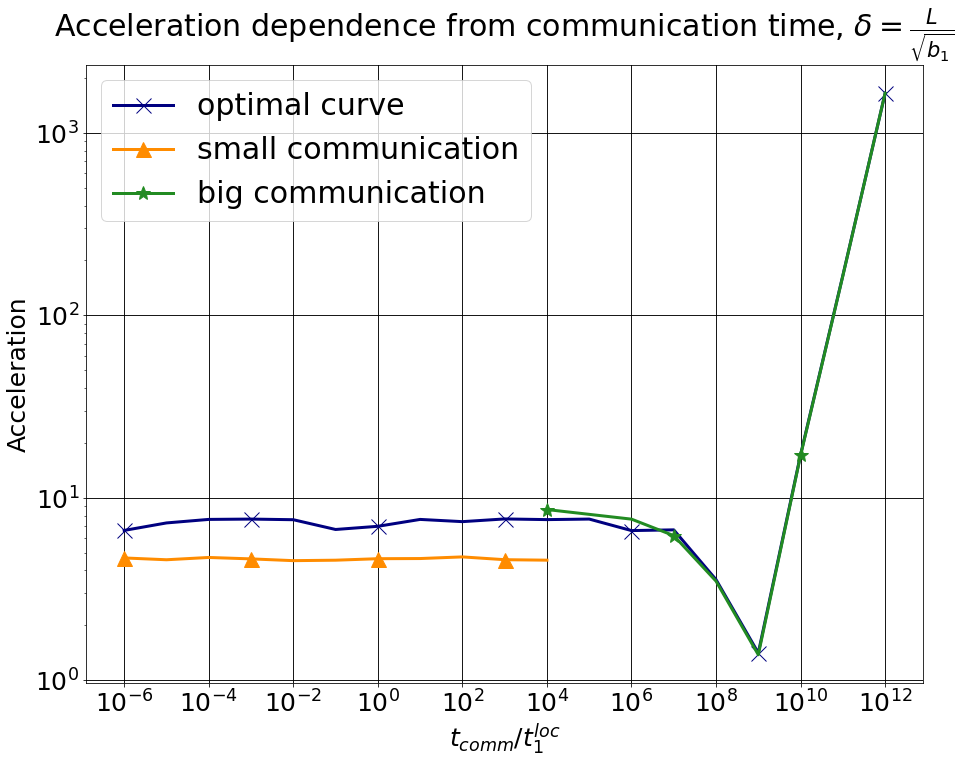
\includegraphics[scale = 0.24]{final_graph1.png}}
    {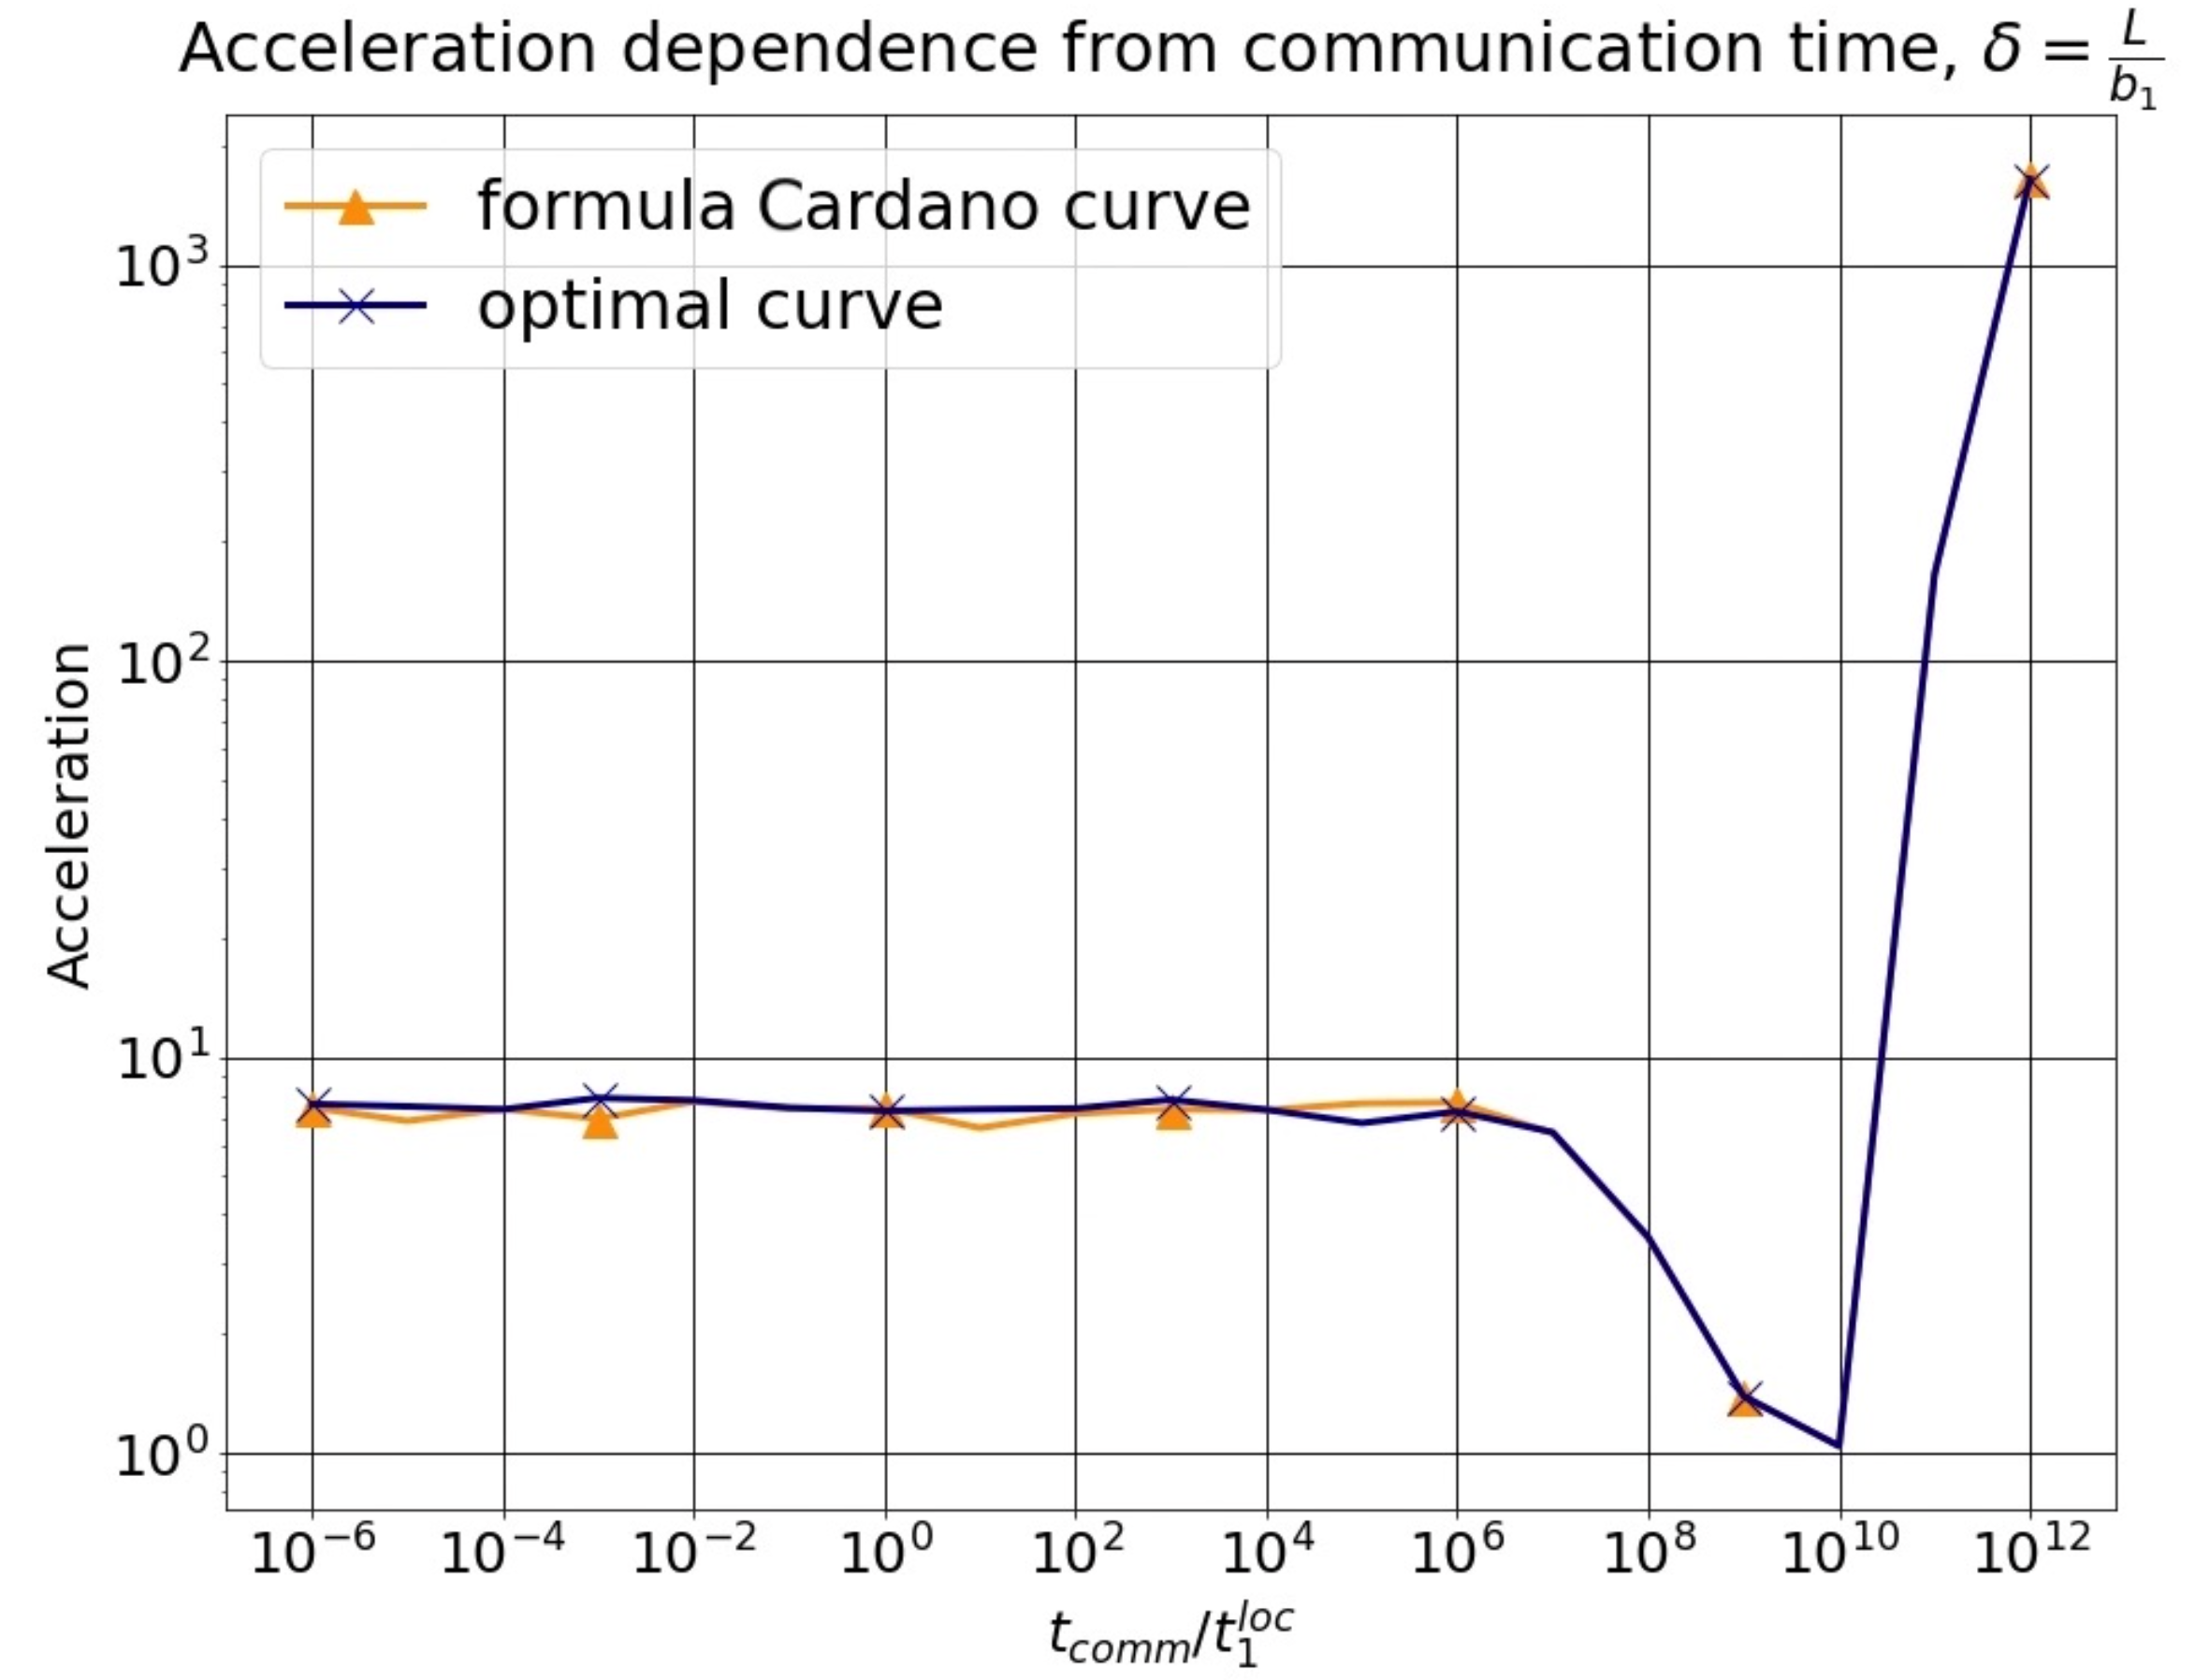
\includegraphics[scale = 0.24]{final_graph2.png}}
    \caption{Final results}
    \label{ris:image}
\end{figure}


%\begin{figure}[h]
%\center{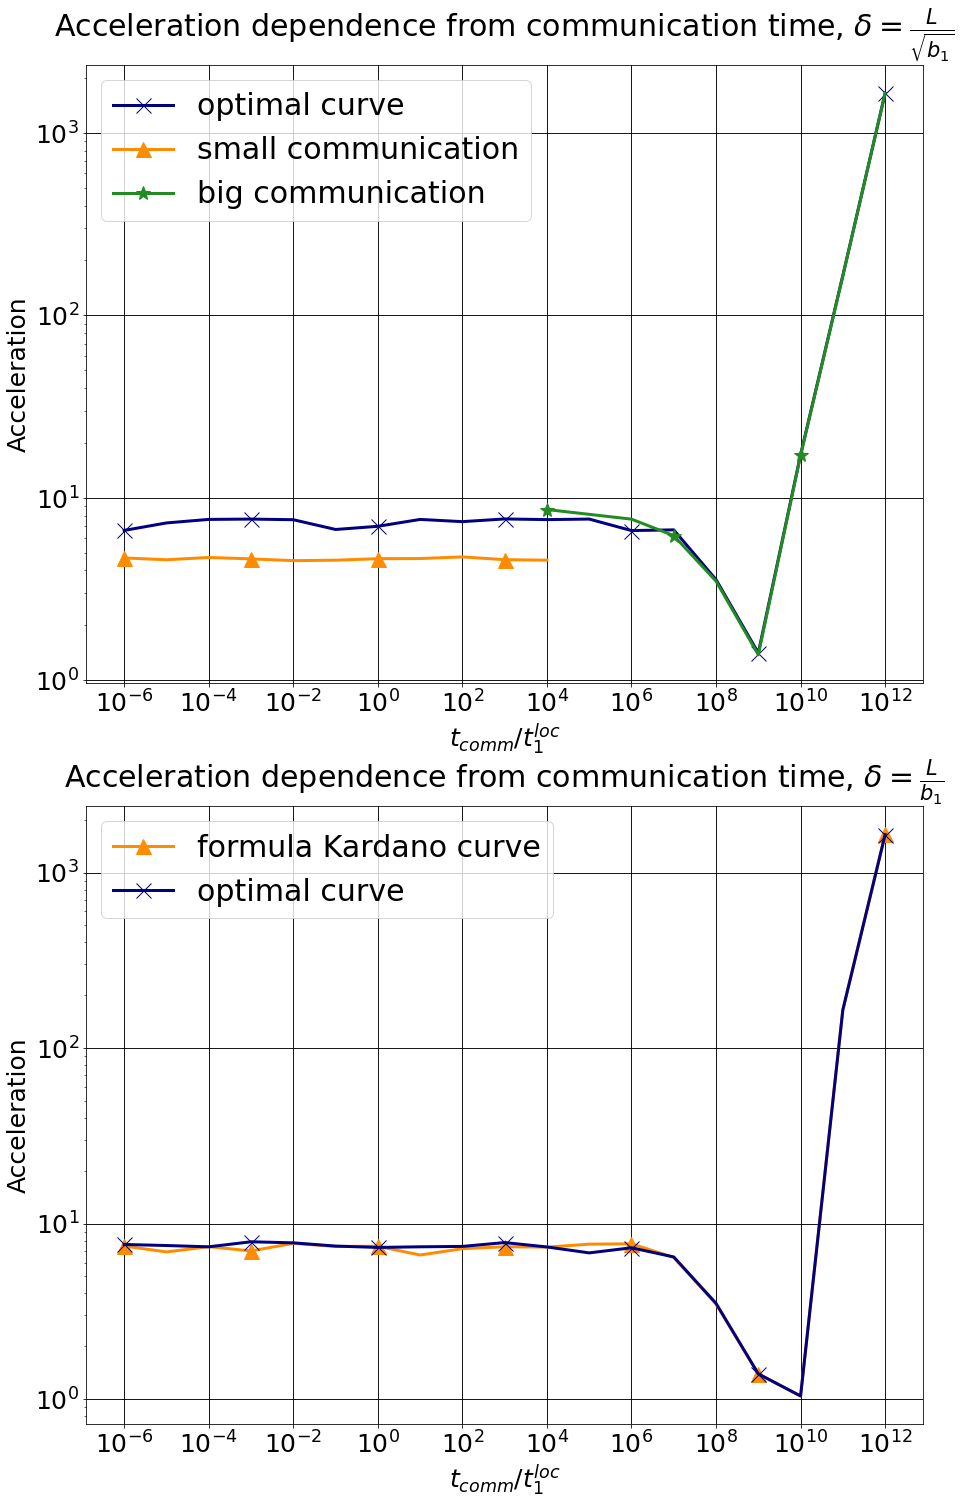
\includegraphics[width=0.8\linewidth]{final_graph.png}}
%\caption{Final results}
%\label{ris:image}
%\end{figure}

\subsection{Analyze}
Let us analyze the obtained graphs. The formula for the case of large communications and the Cardano formula practically coincided with the optimal solution search. The case of small communications showed worse results. This is explained by the fact that the formula was obtained in rough approximation. But if we take into account the constants $\alpha, \beta$, we can get a better result, which is shown below.



\begin{gather*}
    F=\left(\max \left\{\tau_1^{loc} \cdot b_1 ;\left(N-b_1\right) \cdot\left(\sum_{i=2}^n \frac{1}{\tau_i^{loc}}\right)^{-1}\right\}+\tau_{comm}\right) \cdot \frac{\alpha}{\sqrt[4]{b_1}}+\tau_1^{loc} b_1 \cdot \beta, \\
    \text {It has already been evaluated that } b_1 \leq b_1^0 \Rightarrow F=\left(N-b_1\right)\cdot \left(\sum_{i=2}^n \frac{1}{\tau_i^{loc}}\right)^{-1} \cdot \frac{\alpha}{\sqrt[4]{b_1}}+\tau_1^{loc} b_1 \cdot \beta
\end{gather*}


\begin{gather*}
    F=N\left(\sum_{i=2}^n \frac{1}{\tau_i^{loc}}\right)^{-1} \alpha b^{-\frac{1}{4}}-\left(\sum_{i=2}^n \frac{1}{\tau_i^{loc}}\right)^{-1} \alpha b_1^{\frac{3}{4}}+\tau_1^{l o c} \beta b_1 \\
    \text {Consider that} \quad \alpha \sim 10^6, \beta \sim 10^9 \Rightarrow \\ 
    F \cong 10^6 N \left(\sum_{i=2}^n \frac{1}{\tau_i^{loc}}\right)^{-1} \cdot b^{-\frac{1}{4}}-10^6 \left(\sum_{i=2}^n \frac{1}{\tau_i^{loc}}\right)^{-1} \cdot b_1^{\frac{3}{4}}+10^9 \tau_1^{loc} b_1 \\
    \frac{1}{4} 10^6 N \left(\sum_{i=2}^n \frac{1}{\tau_i^{loc}}\right)^{-1} \cdot b_1^{-\frac{5}{4}}=10^5 \tau_1^{loc} \Rightarrow b_1 \cong \frac{4 \cdot 10^3 \tau_1^{loc}}{N\left(\sum_{i=2}^n\left(\tau_i^{loc}\right)^{-1}\right)^{-1}}
\end{gather*}

\section{Conclusion}

In this paper we presented a new way to partition the data for the distributed optimization problem. Our solution is based on separating convex and non-convex subproblems and applying the accelerated extragradient algorithm from \citep{kovalev2022optimal} as well as the OGM-G algorithm from \citep{kim2021optimizing}. Our method works well on star topology networks with various communication costs between the server and the local machines. The theoretical results have been confirmed experimentally. This indicates that our method gives acceleration on tasks of this type.

\bibliographystyle{plain}
\bibliography{refs}  


\end{document}